\documentclass[11pt,a4paper]{article}

\usepackage[margin=2.5cm]{geometry}
\usepackage{amsmath,amssymb}
\usepackage{bm}
\usepackage{graphicx}
\usepackage{booktabs}
\usepackage{xcolor}
\usepackage[colorlinks=true,linkcolor=blue!60!black,urlcolor=blue!60!black]{hyperref}
\usepackage{cleveref}
\usepackage[section]{placeins}

\title{The Kicked Top in Three Regimes\\[0.3em]
  \large Classical phase space, a qubit realisation and its time reversal}
\author{}
\date{}

\begin{document}
\maketitle

\begin{abstract}
The same kicked top is studied in three regimes, regular, mixed and chaotic, selected by the free rotation angle
$p$ at fixed kick strength $k$. Classically, the regimes are read off from Poincar\'e sections and explained with a
small-$p$ reduction of the map to the standard map. Quantum mechanically, the top of spin $j=n_q/2$ is realised by
$n_q$ qubits: the free rotation is a rotation of every qubit and the kick $J_z^2$ is a static all-to-all Ising
coupling. Because the coupling has an integer spectrum, letting it act for a time $2\pi+\varepsilon$ gives the kick, and
letting it act for $2\pi-\varepsilon$ undoes it. This turns a forward evolution into an exact time reversal. The
regimes are compared through the Husimi distribution, the fidelity and the entanglement of a single qubit.
\end{abstract}

\tableofcontents

%=====================================================================
\section{The model}\label{sec:model}
%=====================================================================

A spin $\bm J=(J_x,J_y,J_z)$ of length quantum number $j$ (so $\bm J^2=j(j+1)$, $\hbar=1$) rotates freely about the
$y$ axis and is kicked once per unit time by a torsion about the $z$ axis:
\begin{equation}\label{eq:H}
  H(t) = p\,J_y + \frac{k}{2j}\,J_z^2\sum_{n=-\infty}^{\infty}\delta(t-n).
\end{equation}
Here $p$ is the rotation angle per period (the free rotation velocity), $k$ the kick strength and $\delta$ the
Dirac delta. Integrating the Schr\"odinger equation over one period, starting just after a kick, the free part acts
for unit time and the kick acts instantaneously. One period is therefore the Floquet operator
\begin{equation}\label{eq:U}
  U = e^{-i\frac{k}{2j}J_z^2}\,e^{-ipJ_y},\qquad \psi(t) = U^t\psi(0),\quad t=0,1,2,\dots
\end{equation}
where $t$ now counts periods.

\paragraph{Classical limit.}
The classical top is the same Hamiltonian for a classical vector $\bm J$. All results depend only on the direction
\begin{equation}
  \bm s = \frac{\bm J}{j} = (X,Y,Z) = (\sin\theta\cos\phi,\ \sin\theta\sin\phi,\ \cos\theta),
\end{equation}
a point on the unit sphere with polar angle $\theta$ and azimuth $\phi$. The pair $(\phi,Z)$ is canonical, so phase
space is the rectangle $-\pi<\phi\le\pi$, $-1\le Z\le 1$ with area $4\pi$, and areas in it are conserved. Over one
period the free motion rotates $\bm s$ about $y$ by $p$:
\begin{equation}\label{eq:rot}
  X' = X\cos p + Z\sin p,\qquad Y' = Y,\qquad Z' = -X\sin p + Z\cos p .
\end{equation}
The kick then rotates it about $z$ by the angle $kZ'$, which leaves $Z$ unchanged:
\begin{equation}\label{eq:kick}
  Z_{t+1} = Z',\qquad \phi_{t+1} = \phi' + kZ' ,
\end{equation}
where $\phi'$ is the azimuth of $(X',Y')$. The classical map is \cref{eq:rot,eq:kick}. Its quantum counterpart is
\cref{eq:U}, and $1/j$ plays the role of Planck's constant.

Throughout, $k=20$ (the value that the qubit realisation of \cref{sec:qubits} gives for $n_q=10$ qubits) and only $p$ is
varied:
\begin{equation}
  p = 0.02\ \text{(regular)},\qquad p = 0.1\ \text{(mixed)},\qquad p = 1\ \text{(chaotic)}.
\end{equation}
The initial state is always the north pole $Z=1$ (all spin up).

%=====================================================================
\section{Classical phase space}\label{sec:classical}
%=====================================================================

\Cref{fig:sections} shows Poincar\'e sections: the points $(\phi_t,Z_t)$ of many orbits started on a grid. The red
orbit starts at the pole.

\begin{figure}[h]
  \centering
  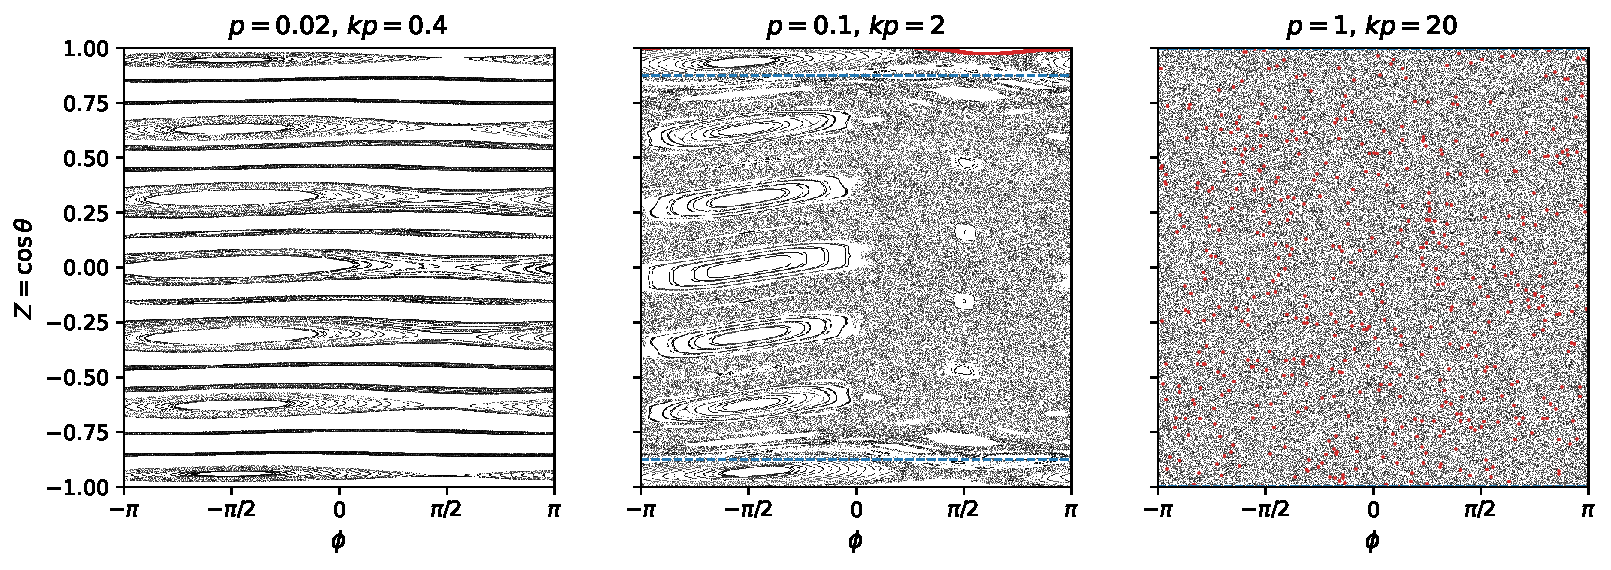
\includegraphics[width=\textwidth]{figures/three_regimes_sections.pdf}
  \caption{Poincar\'e sections at $k=20$, 500 kicks of 400 orbits started on a grid (black), and the orbit started
  at the pole $Z=1$ (red). Dashed: the estimate $|Z|=Z_c$ of \cref{eq:Zc} for the border of the chaotic band.}
  \label{fig:sections}
\end{figure}

\subsection{Small \texorpdfstring{$p$}{p}: the standard map}\label{sec:standard}

For $p\ll1$, \cref{eq:rot} gives to first order in $p$, with $X=\sqrt{1-Z^2}\cos\phi$,
\begin{equation}
  Z' = Z - p\sqrt{1-Z^2}\cos\phi .
\end{equation}
The azimuth also changes by an amount of order $p$, but that is negligible next to the kick angle $kZ'$, which is of
order $k\gg1$. Writing $I=kZ$, the map \cref{eq:rot,eq:kick} becomes
\begin{equation}\label{eq:standard}
  I_{t+1} = I_t - K\cos\phi_t,\qquad \phi_{t+1} = \phi_t + I_{t+1},\qquad K = kp\sqrt{1-Z^2}.
\end{equation}
$Z$ changes by at most $p$ per kick, so $K$ is constant over many kicks and \cref{eq:standard} is, locally in $Z$,
Chirikov's standard map with stochasticity parameter $K$. ($\phi\to\phi+\pi/2$ brings it to the textbook form.) The
strongest kick, $K=kp$, is at the equator, and $K\to0$ at the poles.

\paragraph{Resonances.}
Fixed points of \cref{eq:standard} need $I_{t+1}=I_t$ up to $2\pi$, i.e.\ $\cos\phi=0$, and $\phi_{t+1}=\phi_t$ up to
$2\pi$, i.e.\ $I=2\pi m$ with integer $m$. They lie at
\begin{equation}\label{eq:res}
  Z_m = \frac{2\pi m}{k},\qquad \phi = \pm\frac{\pi}{2},
\end{equation}
a row of resonances spaced by $2\pi/k\approx0.31$. These are the chains of islands in the left panel of
\cref{fig:sections}. A small displacement $(\delta I,\delta\phi)$ from a fixed point evolves as
\begin{equation}
  \begin{pmatrix}\delta I\\ \delta\phi\end{pmatrix}_{t+1} =
  \begin{pmatrix}1 & K\sin\phi\\ 1 & 1+K\sin\phi\end{pmatrix}
  \begin{pmatrix}\delta I\\ \delta\phi\end{pmatrix}_{t}.
\end{equation}
The matrix has determinant 1 (the map preserves area), so its eigenvalues $\lambda$ obey $\lambda^2-T\lambda+1=0$ with
trace $T = 2+K\sin\phi$. For $|T|<2$ they are $e^{\pm i\alpha}$ and the point is stable (the centre of an island). For
$|T|>2$ one of them has $|\lambda|>1$ and the point is unstable. Hence
\begin{equation}
  \phi=-\tfrac{\pi}{2}:\ T=2-K,\ \text{stable for } 0<K<4;\qquad
  \phi=+\tfrac{\pi}{2}:\ T=2+K,\ \text{always unstable}.
\end{equation}
All islands in \cref{fig:sections} sit at $\phi=-\pi/2$, and all chaos starts near $\phi=+\pi/2$.

\paragraph{Width of a resonance.}
Near $I=2\pi m$ let $I = 2\pi m + \Delta$. For small $K$ the map changes $\Delta$ and $\phi$ only a little per kick, so
it is the flow $\dot\Delta = -K\cos\phi$, $\dot\phi = \Delta$ generated by the pendulum Hamiltonian
$\Delta^2/2 + K\sin\phi$. The separatrix passes through the unstable point $\phi=\pi/2$, where the energy is $K$. It is
widest at $\phi=-\pi/2$, where $\Delta^2/2 - K = K$, i.e.\ $\Delta=\pm2\sqrt K$. In $Z$ the island has the full width
$4\sqrt K/k$, and the ratio of width to spacing is
\begin{equation}
  \frac{4\sqrt K/k}{2\pi/k} = \frac{2\sqrt K}{\pi}.
\end{equation}
While this ratio is small, invariant curves running all the way round in $\phi$ survive between neighbouring
resonances (KAM curves), and an orbit cannot cross them. When neighbouring resonances overlap, these curves are
destroyed and orbits wander in $Z$. Setting the ratio to 1 gives $K=\pi^2/4\approx2.5$. Secondary resonances lower the
true threshold, known numerically for the standard map, to
\begin{equation}
  K_c \approx 0.97 .
\end{equation}

\subsection{The three regimes}

Inserting $K = kp\sqrt{1-Z^2}$ into this criterion gives the regimes directly. For the measurements below, the
Lyapunov exponent $\Lambda$ (the growth rate of the distance $d_t\sim e^{\Lambda t}$ between neighbouring orbits) was
computed for a $30\times30$ grid of initial points. A point counts as chaotic if $\Lambda>0.05$.

\begin{description}
\item[Regular, $p=0.02$:] $kp=0.4<K_c$ everywhere. KAM curves separate all resonances, and the motion is regular on the
  whole sphere: $0\%$ of the grid points are chaotic. The orbit from the pole stays at $Z>0.999$.
\item[Mixed, $p=0.1$:] $kp=2$. Chaos needs $K>K_c$, i.e.\ $|Z|<Z_c$ with
  \begin{equation}\label{eq:Zc}
    Z_c = \sqrt{1-\left(\frac{K_c}{kp}\right)^2} \approx 0.87 .
  \end{equation}
  A chaotic band around the equator is bounded by regular caps around the poles (dashed lines in
  \cref{fig:sections}). Inside the band, the islands at $\phi=-\pi/2$ survive because $K<4$. $69\%$ of the grid
  points are chaotic. The orbit from the pole is regular and stays at $Z>0.97$.
\item[Chaotic, $p=1$:] $kp=20\gg K_c$. No KAM curves remain, and except in thin strips at the poles $K>4$, so the
  period-one islands are unstable as well. $100\%$ of the grid points are chaotic, and the orbit from the pole fills the
  sphere.
\end{description}
For $K\gg1$ the standard map stretches by about $K/2$ per kick, i.e.\ $\Lambda\approx\ln(K/2)$. Averaging over the
sphere with $Z$ uniform in $[-1,1]$ (the canonical measure), and using
$\ln\sqrt{1-Z^2}=\tfrac12[\ln(1+Z)+\ln(1-Z)]$ and the symmetry $Z\to-Z$,
\begin{equation}
  \frac12\int_{-1}^{1}\ln\sqrt{1-Z^2}\,dZ = \frac12\int_{-1}^{1}\ln(1+Z)\,dZ = \ln2-1,
\end{equation}
gives
\begin{equation}
  \Lambda \approx \ln\frac{kp}{2} + \ln2 - 1 = \ln(kp) - 1 \approx 2.0
\end{equation}
against the measured mean $1.89$. At $p=1$ the small-$p$ reduction is no longer justified, so this is only an
estimate.

%=====================================================================
\section{Quantum top: phase-space resolution}\label{sec:quantum}
%=====================================================================

The quantum analogue of a phase-space point is the spin coherent state
\begin{equation}
  |\theta,\phi\rangle = e^{-i\phi J_z}e^{-i\theta J_y}|j,j\rangle ,
\end{equation}
the fully polarised state $|j,j\rangle$ ($J_z=j$) rotated to the direction $(\theta,\phi)$. The Husimi distribution of
a state $\psi$,
\begin{equation}\label{eq:Q}
  Q(\theta,\phi) = |\langle\theta,\phi|\psi\rangle|^2 ,\qquad
  \frac{2j+1}{4\pi}\int_{-\pi}^{\pi}\!d\phi\int_{-1}^{1}\!dZ\;Q = 1,
\end{equation}
is the probability of finding $\psi$ in the direction $(\theta,\phi)$, drawn on the same $(\phi,Z)$ plane as the
Poincar\'e sections.

The overlap of two coherent states whose directions make an angle $\gamma$ is
$|\langle\theta,\phi|\theta',\phi'\rangle|^2 = \cos^{4j}(\gamma/2)\approx e^{-j\gamma^2/2}$, so a coherent state is
a spot of angular width $1/\sqrt j$. By \cref{eq:Q} it occupies an area $4\pi/(2j+1)$ of phase space, a ``Planck
cell''. For $j=5$ this is $1.1$ out of $4\pi$, i.e.\ only $2j+1=11$ cells cover the sphere. One resonance strip of
\cref{eq:res} has area $2\pi\times2\pi/k\approx2.0$, about two cells. The quantum top at $j=5$ therefore resolves
the three regimes only coarsely: it sees whether the state stays localised or spreads, but not the individual islands.

%=====================================================================
\section{Qubit realisation}\label{sec:qubits}
%=====================================================================

\subsection{Collective spin of \texorpdfstring{$n_q$}{n\_q} qubits}

Take $n_q$ qubits with Pauli matrices $\sigma^a_i$ ($a=x,y,z$, qubit $i=1,\dots,n_q$) and define
\begin{equation}\label{eq:Jq}
  J_a = \frac12\sum_{i=1}^{n_q}\sigma^a_i .
\end{equation}
Pauli matrices of different qubits commute, and $[\sigma^a_i/2,\sigma^b_i/2]=i\epsilon_{abc}\sigma^c_i/2$, where
$\epsilon_{abc}$ is the Levi-Civita symbol and $c$ is summed over. Hence $[J_a,J_b]=i\epsilon_{abc}J_c$: $\bm J$ is
an angular momentum. The all-up state $|{\uparrow\cdots\uparrow}\rangle$ has $J_z=n_q/2$, the largest possible value,
so it is $|j,j\rangle$ with
\begin{equation}
  j = \frac{n_q}{2}.
\end{equation}
The operator $U$ is built from the $J_a$ alone, so it commutes with $\bm J^2$ and with every permutation of the qubits.
A state that starts in the totally symmetric subspace, of dimension $2j+1$ and containing $|j,j\rangle$, stays in it.
Within this subspace the $2^{n_q}$-dimensional chain is exactly the spin-$j$ top. Starting from the all-up state, the
chain is therefore the quantum top of \cref{sec:quantum} with $j=5$ ($n_q=10$) or $j=6$ ($n_q=12$).

\subsection{Free rotation: single-qubit pulses}

The terms of $J_y$ in \cref{eq:Jq} commute, so the exponential factorises:
\begin{equation}
  e^{-ipJ_y} = \prod_{i=1}^{n_q} e^{-i\frac p2\sigma^y_i}.
\end{equation}
The free rotation is the same rotation by $p$ about $y$, applied to every qubit independently.

\subsection{Kick: all-to-all Ising coupling}

Squaring \cref{eq:Jq} and using $(\sigma^z_i)^2=1$,
\begin{equation}
  J_z^2 = \frac14\sum_{i,l}\sigma^z_i\sigma^z_l = \frac{n_q}{4} + \frac12 H_{zz},\qquad
  H_{zz} = \sum_{i<l}\sigma^z_i\sigma^z_l .
\end{equation}
$H_{zz}$ is a static Ising coupling of unit strength between all pairs of qubits. On a basis state with $u$ qubits up,
$J_z = m = u-n_q/2$ and
\begin{equation}\label{eq:Hzz}
  H_{zz} = 2m^2-\frac{n_q}{2} = 2u(u-n_q)+\frac{n_q(n_q-1)}{2},
\end{equation}
an integer, because $n_q(n_q-1)$ is even. Consequently
\begin{equation}
  e^{-i2\pi H_{zz}} = 1 .
\end{equation}
Let the coupling act for the time $T=2\pi+\varepsilon$. Then
\begin{equation}\label{eq:kickq}
  e^{-iTH_{zz}} = e^{-i\varepsilon H_{zz}} = e^{i\varepsilon n_q/2}\;e^{-i2\varepsilon J_z^2}.
\end{equation}
Apart from a global phase, this is the kick of \cref{eq:U} with $k/(2j)=2\varepsilon$, i.e.
\begin{equation}\label{eq:k}
  k = 4j\varepsilon = 2n_q\varepsilon .
\end{equation}
For $\varepsilon=1$: $k=20$ for $n_q=10$ and $k=24$ for $n_q=12$. One forward period of the chain is
\begin{equation}\label{eq:Uf}
  U_f = e^{-i(2\pi+\varepsilon)H_{zz}}\prod_{i}e^{-i\frac p2\sigma^y_i} ,
\end{equation}
which equals $U$ of \cref{eq:U} up to a phase. Numerically, $\langle\bm J\rangle$ of the chain agrees with the
spin-$j$ top to $10^{-13}$.

\paragraph{Mean-field picture.}
In \cref{eq:kickq}, qubit $i$ feels $\varepsilon\,\sigma^z_i\sum_{l\ne i}\sigma^z_l$, a rotation about $z$ by the angle
$2\varepsilon\sum_{l\ne i}\sigma^z_l$. Replacing the other qubits by their mean, $\sum_{l\ne i}\sigma^z_l\approx
2\langle J_z\rangle = n_qZ$, gives the angle $2n_q\varepsilon Z = kZ$. This is the classical torsion of \cref{eq:kick}:
each qubit precesses in the field of all the others.

%=====================================================================
\section{Time reversal}\label{sec:reversal}
%=====================================================================

To run the evolution backwards one needs $U_f^{-1} = U_f^\dagger$, which contains $e^{+i\varepsilon H_{zz}}$, i.e.\ the
coupling acting for a negative time. The integer spectrum avoids this: by \cref{eq:Hzz}, acting for the positive time
$T'=2\pi-\varepsilon$ is equivalent to acting for $-\varepsilon$. The backward period changes the sign of $p$ and the
order of the two factors:
\begin{equation}\label{eq:Ub}
  U_b = \prod_{i}e^{+i\frac p2\sigma^y_i}\;e^{-i(2\pi-\varepsilon)H_{zz}} .
\end{equation}
Then
\begin{equation}
  U_bU_f = e^{ipJ_y}\,e^{-i4\pi H_{zz}}\,e^{-ipJ_y} = 1 ,
\end{equation}
so $U_b = U_f^\dagger$ exactly, in every regime. In the language of the top, $T\to T'$ is $k\to-k$, achieved without
changing the sign of the coupling.

\paragraph{Protocol.}
Starting from $\psi_0=|{\uparrow\cdots\uparrow}\rangle$, apply $U_f$ for $t_r$ periods and then $U_b$ for $t_r$ periods:
\begin{equation}
  \psi(t) = U_f^{\,t}\psi_0\quad (0\le t\le t_r),\qquad
  \psi(t_r+s) = U_b^{\,s}U_f^{\,t_r}\psi_0 = U_f^{\,t_r-s}\psi_0 = \psi(t_r-s)\quad(0\le s\le t_r).
\end{equation}
Two consequences follow. The state returns, $\psi(2t_r)=\psi_0$. And every quantity is mirror-symmetric about $t_r$:
its value at $t_r+s$ equals its value at $t_r-s$. Without imperfections the echo is perfect in all three regimes, so the
regimes differ only in what happens between $0$ and $2t_r$. Here $t_r=30$.

\paragraph{Measures.}
The fidelity
\begin{equation}
  F(t) = |\langle\psi_0|\psi(t)\rangle|^2
\end{equation}
is the probability of finding the initial state again. For a state spread evenly over the $2j+1$ symmetric states it
is about $1/(2j+1)$.

By permutation symmetry, every qubit has the same Bloch vector, $\langle\bm\sigma_i\rangle = \langle\bm J\rangle/j$.
The reduced state of one qubit is $\rho_i = (1+\langle\bm\sigma_i\rangle\cdot\bm\sigma)/2$ with purity
$\operatorname{Tr}\rho_i^2 = (1+r^2)/2$, where
\begin{equation}
  r = |\langle\bm\sigma_i\rangle| = \frac{|\langle\bm J\rangle|}{j}.
\end{equation}
Since the whole chain is in a pure state, $r=1$ means qubit $i$ is unentangled with the rest, and $r<1$ means it is
entangled. $r$ is thus both the length of the classical vector $\bm s$ seen by the quantum state and a measure of the
entanglement created by the coupling. The total spin $\langle\bm J^2\rangle = j(j+1)=30$ is conserved throughout.

\subsection{Results}

\begin{figure}[h]
  \centering
  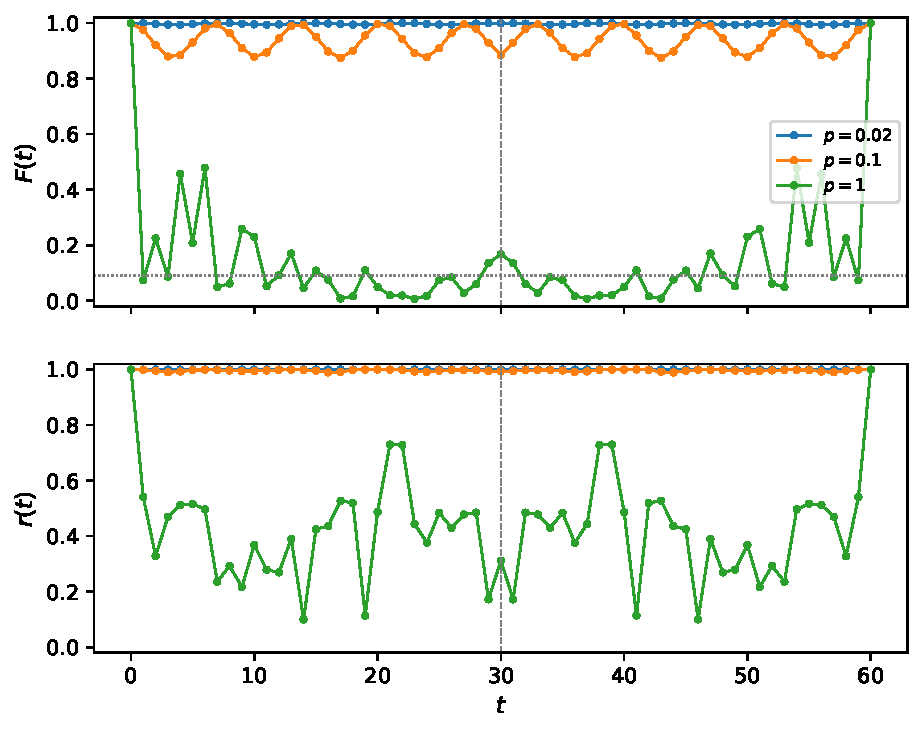
\includegraphics[width=0.8\textwidth]{figures/three_regimes_echo.pdf}
  \caption{Fidelity $F(t)$ (top) and single-qubit Bloch-vector length $r(t)$ (bottom) for $n_q=10$, $\varepsilon=1$
  ($k=20$), reversal at $t_r=30$ (dashed). Dotted: $1/(2j+1)$.}
  \label{fig:echo}
\end{figure}

\begin{figure}[h]
  \centering
  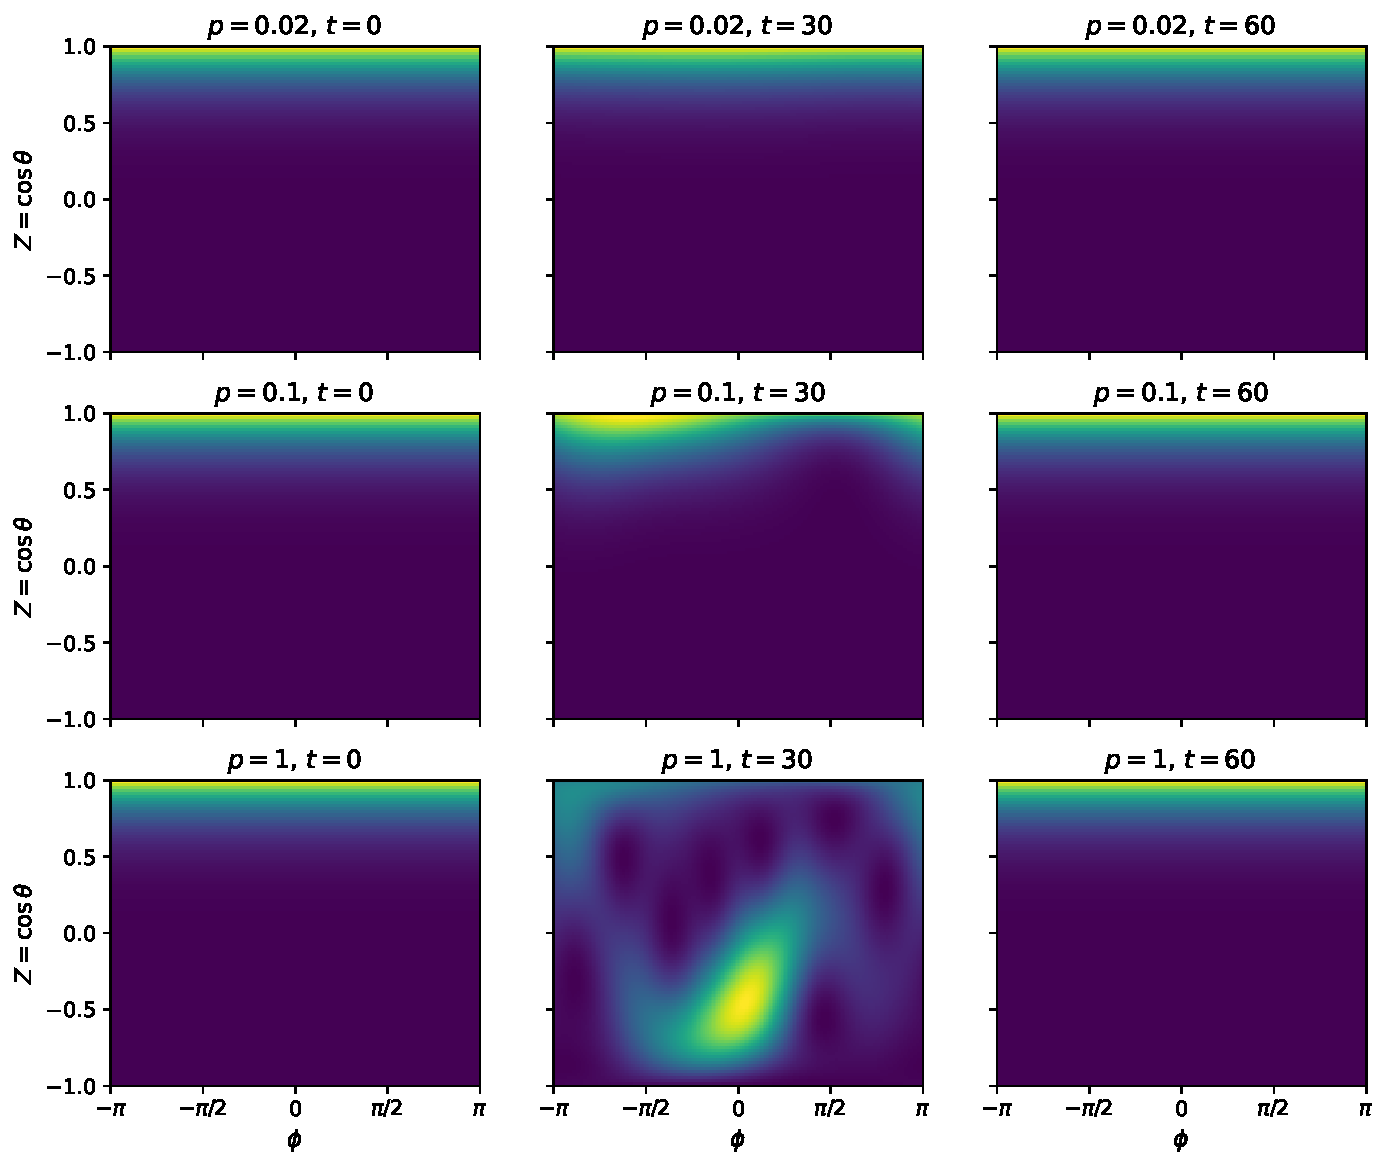
\includegraphics[width=\textwidth]{figures/three_regimes_husimi.pdf}
  \caption{Husimi distribution \cref{eq:Q} of the chain state at $t=0$, $t_r$ and $2t_r$, for the three values of $p$.}
  \label{fig:husimi}
\end{figure}

\begin{description}
\item[Regular, $p=0.02$:] The pole lies in the regular region, and the classical orbit stays within $Z>0.999$, far
  inside one Planck cell. The state barely moves: $F\ge0.994$ and $r\ge0.99998$. The Husimi distribution at $t_r$ is
  indistinguishable from the initial one.
\item[Mixed, $p=0.1$:] The pole lies in the regular polar cap $Z>Z_c$. The state stays localised there but oscillates
  around the regular orbit: $F$ oscillates between $0.87$ and $1$, and $r\ge0.989$, so almost no entanglement is
  created. The Husimi distribution at $t_r$ is deformed but stays in the cap.
\item[Chaotic, $p=1$:] The state spreads after one kick, with $F(1)=0.07$. This agrees with the time over which a
  coherent state follows the classical orbit, about $\ln j/(2\Lambda)\approx0.4$ kicks. Afterwards $F$ fluctuates
  around $0.1\approx1/(2j+1)$. $r$ drops to $0.1$–$0.3$, so each qubit is strongly entangled with the rest. At $t_r$
  the Husimi distribution is no longer a single coherent spot: its maximum drops from $0.95$ to $0.45$, it lies far
  from the pole (near $Z\approx-0.45$), and it is spread over about 5 of the 11 Planck cells, i.e.\ half of the
  sphere. (The number of cells is $(2j+1)\,(\int Q)^2/(4\pi\int Q^2)$ with $\int=\int d\phi\,dZ$, which gives
  about 2 for a coherent state.)
\end{description}
In all three regimes the backward leg mirrors the forward one, and $F(2t_r)=1$ and $Q(2t_r)=Q(0)$ hold to
$10^{-13}$ (\cref{fig:echo,fig:husimi}).

\end{document}
